\subsection{Voronoi-Diagramme}
\begin{description}
	\item[Problem:] ``Telefonzellenproblem'':
		\begin{description}
			\item[gesucht:] eine Unterteilung der Ebene in $n$ (Anzahl von Knoten) Zellen mithilfe einer Distanzfunktion $d:\mathbb{R}^2 \rightarrow \mathbb{R}_{\geq 0}$
			\item[mathematisch:] $V(p_i) = \{p \in \mathbb{R}^2; d(p,p_i) \leq d(p,p_j), j=1,\dots,n\},~~i=1,\dots,n$
		\end{description}
\end{description}
\begin{itemize}
	\item Distanzfunktion $d$ ist die euklidische Distanz:\\
		$d\left(\aoverb{x_1}{y_1},\aoverb{x_2}{y_2}\right) = \sqrt{(x_1-x_2)^2+(y_1-y_2)^2}$
	\item $V(p_1),\dots,V(p_n)$ sind \textit{Voronoi-Zellen}
	\item ein Voronoi-Diagramm $Vor(P)$ besteht aus den Grenzen der Voronoi-Zellen
	\item Knoten $V$ von $Vor(P)$ sind die Punkte, die auf den Grenzen von mindestens drei Zellen liegen
	\item Kanten $E$ von $Vor(P)$ sind die verbundenen Teilmengen von $Vor(P)$ ohne $V$
	\item manche Kanten von $Vor(P)$ können unendliche Länge haben
	\item Knoten aus $P$ bezeichnen wir als \site s
	\item ein Punkt $p$ ist ein Knoten in $Vor(P) \Longleftrightarrow p$ ist Zentrum eines Kreises mit mindestens drei \site s~auf seinem Umkreis und keiner \site~innerhalb des Kreises
	\item ein Punkt $p$ ist auf einer Kante in $Vor(P) \Longleftrightarrow p$ ist Zentrum eines Kreises mit genau zwei \site s~auf seinem Umkreis und keiner \site~innerhalb des Kreises
	\item eine Voronoi-Zelle eines Punktes $p_i,i=1,\dots,n$ kann wie folgt konstruiert werden:
		\begin{itemize}
			\item für alle $p_j,j\neq i$ teilt die Mittelsenkrechte $\oben{p_ip_j}$ die Fläche in zwei Halbebenen
			\item $H_{p_j}(p_i)$ ist die Halbfläche, die $p_i$ enthält\\
			$\Rightarrow V(p_i) = \bigcap\limits_{j\neq i} H_{p_j}(p_i)$
		\end{itemize}
	\item wenn das Voronoi-Diagramm auf diese Weise konstruiert wird, müssen die Schnittpunkte der $n-1$ Mittelsenkrechten berechnet werden, allerdings ist die Anzahl der Knoten und Kanten linear zur Anzahl der \site s
\end{itemize}
\begin{description}
	\item[Lemma:] Ein Voronoi-Diagramm einer Menge vin $n\geq 3$ \site s hat höchstens $2n-5$ Knoten und $3n-6$ Kanten
	\up\Proof
	\up\begin{itemize}
		\item Annahme: alle \site s liegen auf einer Linie\\
			$\Rightarrow$ Voronoi-Diagramm besteht aus $n-1$ parallelen Linien\\
			$\Rightarrow$ $n-1$ Kanten, keine Knoten
		\item sonst ist das Diagramm verbunden und alle Kanten sind Segmente oder Halblinien
		\item zur Betrachtung des Diagramms als normalen planaren Graphen:
			\begin{itemize}
				\item Hinzufügen eines Knotens $v_{\infty}$ als künstlicher Endknoten der Halblinien
				\item beinhaltet dann einen planaren verbundenen Graphen mit $n$ Flächen, gleich vielen Kanten wie das Voronoi-Diagramm und einem Knoten mehr als das Voronoi-Diagramm
				\item mir der eulerschen Formel erhalten wir: $\#$Flächen $=f = |E|-|V|+1+k$, wobei $k$ der Anzahl der Zusammenhangskomponenten entspricht (bei einem verbundenen Graphen gilt $k=1$)
				\item jede Kante ist inzident zu zwei Knoten
				\item jeder Knoten (auch $v_{\infty}$) ist mindestens zu drei Kanten inzident\\
				$\Rightarrow 2\cdot |E| \geq 3\cdot |V| \Longrightarrow |V| \leq \dfrac{2}{3}\cdot |E| \Longrightarrow n = |E|-|V|+1+k \geq |E|-\dfrac{2}{3}\cdot |E|+2\\
				\Longrightarrow |E|\leq 3n -6 \Longrightarrow |V|\leq \dfrac{2}{3}|E| \leq 2n -4$
			\end{itemize}
	\end{itemize}
\end{description}
\topbreak
\up\up\up
\begin{description}
	\item[]\ \\\up
		\begin{itemize}
			\item da $V$ den fiktiven Knoten $v_{\infty}$ enthält, wissen wir jetzt, dass ein Voronoi-Diagramm höchstens $|V|-1 \leq 2n-5$ Knoten enthält
		\end{itemize}
\end{description}
\begin{itemize}
	\item \begin{description}
			\item[Algorithmus von Fortune:] zur Einfachheit nehmen wir an, dass es keinen Kreis gibt mit vier \site s auf seinem Umkreis und kein \site~in seinem Inneren \\\up
				\begin{description}
					\item[\sweep~Status:] \ \\\up
						\begin{itemize}
							\item jeder Punkt, der näher zu einem Punkt links der \sweep~$l$ ist als zu $l$ selbst, kann nicht in einer Voronoi-Zelle einer \site~sein, die rechts der \sweep~liegt
							\item die \textbf{\beach}~ist eine Kurve, die die Menge der Punkte, die näher zu einem Punkt links von $l$ als zu $l$ selbst sind, von den Punkten, die näher an $l$ sind, trennt
							\item die \beach~ist \textbf{y-monoton} (d.h. jede horizontale Linie schneidet die \beach~in genau einem Punkt)
							\item wenn es genau eine \site~links der \sweep~gibt, dann ist die \beach~eine (gedrehte) Parabel
							\item allgemein: die \beach~ist eine Sequenz von Parabelbögen, wobei jeder Bogen zu einer \site~gehört
							\item manche Parabel können mehrere Teile der Teilstrecken der \beach~beisteuern
							\item ein Schnittpunkt zwischen zwei aufeinanderfolgenden Parabelbögen auf der \beach~wird \textbf{\bpoint} genannt
							\item der Status der \sweep~ist die geordnete Sequenz von Parabelbögen und \bpoint s auf der \beach
							\item Speicherung des \sweep~Status in einem binären Suchbaum
						\end{itemize}
						\example{\beach~\&~\text{binärer Suchbaum}}{\ \\\up
						\begin{minipage}{0.2\textwidth}
							\includegraphics[scale=0.25]{Pics/8_beachline-tree.png}
						\end{minipage}
						\hfill
						\begin{minipage}{0.75\textwidth}
						Baum vor dem Einfügen von $p_6$:\\
						\resizebox{0.7\textwidth}{!}{
							\input{Pics/8_treeBefore.pgf}}
						\end{minipage}\\\\\\
						\begin{minipage}{0.4\textwidth}
						Baum nach dem Einfügen von $p_6$:
						\end{minipage}
						\hfill
						\begin{minipage}{0.5\textwidth}
						Baum nach der Neuausrichtung:
						\end{minipage}\\
						\begin{minipage}{0.4\textwidth}
						\resizebox{\textwidth}{!}{
							\input{Pics/8_treeAfter.pgf}}
						\end{minipage}
						\hfill
						\begin{minipage}{0.5\textwidth}
						\resizebox{0.8\textwidth}{!}{
							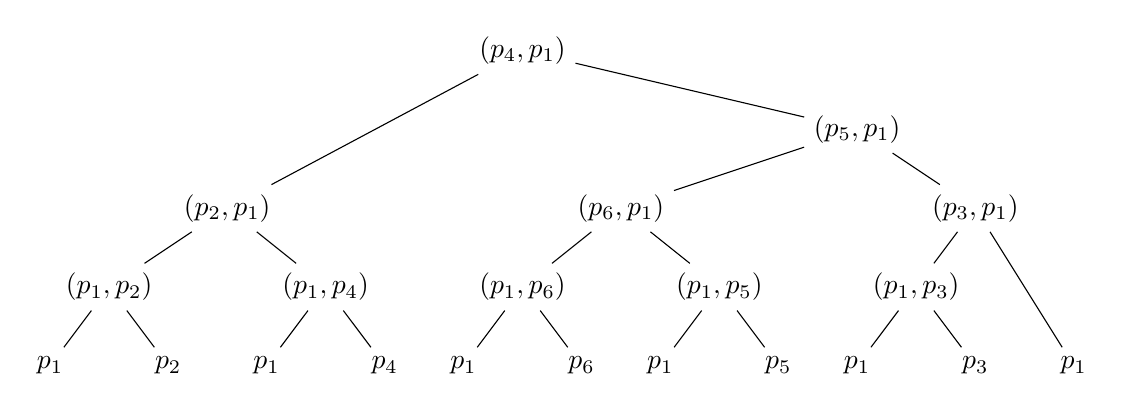
\begin{tikzpicture}
\node at (0,0) {$(p_4,p_1)$}
	child[xshift=-3cm,yshift=-0.5cm] {node {$(p_2,p_1)$}
		child[xshift=-0.75cm,yshift=0.5cm] {node {$(p_1,p_2)$}
			child[yshift=0.5cm] {node {$p_1$}}
			child[yshift=0.5cm] {node {$p_2$}}
		}
		child[xshift=0.5cm,yshift=0.5cm] {node {$(p_1,p_4)$}
			child[yshift=0.5cm] {node {$p_1$}}
			child[yshift=0.5cm] {node {$p_4$}}
		}
	}
	child[xshift=3.5cm,yshift=0.5cm] {node {$(p_5,p_1)$}
		child[xshift=-2.25cm,yshift=0.5cm] {node {$(p_6,p_1)$}
			child[xshift=-0.5cm,yshift=0.5cm] {node {$(p_1,p_6)$}
				child[yshift=0.5cm] {node {$p_1$}}
				child[yshift=0.5cm] {node {$p_6$}}
			}
			child[xshift=0.5cm,yshift=0.5cm] {node {$(p_1,p_5)$}
				child[yshift=0.5cm] {node {$p_1$}}
				child[yshift=0.5cm] {node {$p_5$}}
			}
		}
		child[xshift=0.75cm,yshift=0.5cm] {node {$(p_3,p_1)$}
			child[yshift=0.5cm] {node {$(p_1,p_3)$}
				child[yshift=0.5cm] {node {$p_1$}}
				child[yshift=0.5cm] {node {$p_3$}}
			}
			child[xshift=0.5cm,yshift=-0.5cm] {node {$p_1$}}
		}
	}
;
\end{tikzpicture}}
						\end{minipage}\\\ \\
						}
				\end{description}
		\end{description}
\end{itemize}
\topbreak
\up\up
\begin{itemize}
	\item[] \begin{description}
			\item[]\ \\\up\up \begin{description}
					\item[Ereigniszeitplan:]\ \\\up
						\begin{itemize}
							\item der Status der \sweep~ändert sich, wenn ein neuer Parabelbogen auf der \beach~auftaucht bzw. wenn ein Parabelbogen von der \beach~verschwindet
							\item verwendete Datenstruktur: \PQ
						\end{itemize}
						\begin{description}
							\item[\site-Event:]\ \\\up
								\begin{minipage}{0.5\textwidth}
									\begin{itemize}
										\item ein neuer Parabelbogen kann \textbf{nur} dann auf der \beach~auftauchen, wenn die \sweep~einen \site~$p$ enthält
										\item somit sind alle \site s, sortiert in nicht-absteigender Reihenfolge ihrer $x$-Koordinate eine Teil-Sequenz des Ereigniszeitplans
										\item Einfügen eines neuen Parabelbogens in den Suchbaum:
									\end{itemize}
								\end{minipage}\hfill
								\begin{minipage}{0.3\textwidth}
									\includegraphics[width=\textwidth]{Pics/8_siteevent.png}
								\end{minipage}\\
								\begin{itemize}
									\item[] \begin{enumerate}
											\item traversieren des Suchbaums
											\item am Ende wird die $y$-Koordinate von $p$ mit der Koordinate der Positionen der aktuellen \bpoint~verglichen
											\item die Suche endet im Parabelbogen $\alpha$ links von $p$
										\end{enumerate}
									\item $q$ ist das Label von $\alpha$
									\item $\alpha$ ist ein Fragment der Parabel, welches die Punkte näher bei der \site~$q$ von den Punkten, die näher bei der \sweep~liegen trennt
									\item Ersetzten von $\alpha$ in Suchbaum durch einen Teilbaum, der die Sequenz $q,(q,p),p(p,q),q$ von drei Parabelbögen und ihren \bpoint s repräsentiert (Parabelbögen sind die Blätter)
									\item $p$ kann direkt rechts von einem \bpoint~liegen:
										\begin{enumerate}
											\item Aufteilen von $\alpha$ in zwei Teile, wobei ein Teil die Länge $0$ hat
											\item dieser Bogen mit Länge $0$ wird sofort als verschwindender Bogen betrachtet
										\end{enumerate}
								\end{itemize}
							\item[\kreis:]\ \\\up
								\begin{minipage}{0.5\textwidth}
									\begin{itemize}
										\item ein Parabelbogen $\alpha$ mit Label $q$ verschwindet dann aus dem \sweep~Status, wenn der \bpoint~$(p_1,q)$ unter $\alpha$ mit dem \bpoint~$(q,p_2)$ über $\alpha$ übereinstimmt\\
										$\Rightarrow$ der Punkt $p_0$, an dem $\alpha$ verschwindet, ist der Punkt auf der \beach, der gleich weit entfernt ist von den \site s $p_1,q,p_2$, wie zu der \sweep\\
										$\Rightarrow p_0$ ist das Zentrum eines Kreises, der die \sweep~berührt, die \site s $p_1,q,p_2$ sind auf seinem Umkreis und kein \site~liegt innerhalb
									\end{itemize}
								\end{minipage}\hfill
								\begin{minipage}{0.3\textwidth}
									\includegraphics[width=\textwidth]{Pics/8_circleevent.png}
								\end{minipage}\\
								\begin{itemize}
									\item ein Parabelbogen $\alpha$ wird nicht verschwinden, falls ein Parabelbogen direkt über und unter $\alpha$ die gleiche \site~als Label haben
									\item ein Punkt ist der Ort, an dem ein Parabelbogen verschwindet\\ $\Longleftrightarrow$ der Punkt ist ein Knoten im Voronoi Diagramm
									\item um ein \kreis~in den Ereigniszeitplan einzubinden tun wir folgendes:
										\begin{enumerate}
											\item an jedem Ereignispunkt gilt: die drei Parabelbögen mit den Labeln $p_1,p_2,p_3$ erscheinen neu auf der \beach
											\item bei einem \site~liegt einer der drei oben genannten Bögen auf der \sweep, bei einem \kreis~ist gerade ein Bogen verschwunden bei $(p_1,p_2)$ oder bei $(p_2,p_3)$
											\setcounter{temp}{\value{enumi}}
										\end{enumerate}
								\end{itemize}
						\end{description}
				\end{description}
		\end{description}
\end{itemize}
\topbreak
\up\up\up\up
\begin{itemize}
	\item[] \begin{description}
			\item[]\ \\\up\up \begin{description}
					\item[]\ \\\up
						\begin{description}
							\item[]\ \\\up
								\begin{minipage}{0.84\textwidth}
									\begin{itemize}
										\item[]
											\begin{enumerate}
											\setcounter{enumi}{\value{temp}}
												\item azwei \bpoint s $(p_1,p_2)$ und $(p_2,p_3)$ konvergieren, wenn
													\begin{enumerate}
														\item $p_1\neq p_3$,
														\item $p_1,p_2,p_3$ liegen nicht auf einer Linie und
														\item der rechteste Punkt $r$ eines eindeutigen Kreises durch $p_1,p_2,p_3$ ist rechts der aktuellen \sweep, oder $r$ ist die \site, die gerade rechts von einem \bpoint~eingefügt wurde
													\end{enumerate}
											\end{enumerate}
										\item wenn zwei \bpoint s konvergieren, wird ein ``potentieller'' \kreis~in den Ereigniszeitplan eingefügt
										\vspace*{-0.5\baselineskip}
										\item ein \kreis~bei $r$ kann ein falscher Alarm gewesen sein (kann passieren, wenn die Bögen $p_1$ oder $p_3$ nicht vor $p_2$ durch ein \kreis~verschwindet, oder weil $p_1,p_2$ oder $p_3$ in zwei Teile durch ein \site-Event aufgeteilt wurde)
										\vspace*{-0.5\baselineskip}
										\item im letzten Fall wird der der \kreis~wieder aus dem Ereigniszeitplan entfernt
										\vspace*{-0.5\baselineskip}
										\item hierfür speichern werden die Zeiger der Parabelbögen zu den \kreis~gespeichert, in denen sie beteiligt waren
										\vspace*{-0.5\baselineskip}
										\item zum Löschen eines verschwundenen Parabelbogens $\alpha$ aus dem Suchbaum, wird ein Zeiger vom \kreis~zu $\alpha$ verwendet:
											\begin{enumerate}
												\item Löschen von $\alpha$
												\item falls $\alpha$ nicht beides hat (Vorgänger und Nachfolger) im \sweep~Status (beides wären \bpoint, falls es sie gibt): Löschen des bestehenden (Vorgänger oder Nachfolger) aus dem Suchbaum
												\item sonst: Löschen des Vorgängers von $\alpha$ und Ersetzen des Nachfolgers von $\alpha$ mit dem \bpoint~zwischen dem Parabelbogen direkt unter $\alpha$ und dem Parabelbögen direkt über $\alpha$
												\item die einzige Änderung im Suchbaum während einer Löschoperation ist, dass das gelöschte Element durch seinen Nachfolger ersetzt wird
												\item da $\alpha$ schon gelöscht wurde, kann höchstens der Vorgänger von $\alpha$ durch den Nachfolger von $\alpha$ ersetzt werden
												\item Eigenschaft der inneren Knoten des Suchbaums (die \bpoint s) bleibt erhalten
											\end{enumerate}
									\end{itemize}
								\end{minipage}\\\\
						\end{description}
				\end{description}
		\end{description}
	\item \begin{description}
			\item[Konstruktion des Voronoi-Diagrammes:]\ \\\up\up
				\begin{itemize}
					\item Algorithmus mit der \sweep~basiert auf:\vspace*{-0.5\baselineskip}
						\begin{enumerate}
							\item ein Punkt ist ein Knoten in einem Voronoi-Diagramm $\Longleftrightarrow$ der Punkt ist das Zentrum eines \kreis
							\vspace*{-0.5\baselineskip}
							\item die \bpoint s stecken die Kanten des Voronoi-Diagrammes ab
						\end{enumerate}
					\up\item Speicherung des Voronoi-Diagrammes: doppelt-verkettete Kantenliste verwendet
					\vspace*{-0.5\baselineskip}\item immer, wenn ein neuer \bpoint~in die \beach~eingefügt wird, erstellen wir zwei neue Kanten $e$ und $Twin(e)$, mit den zugehörigen \site s der \bpoint s als ihre inzidenten Flächen
					\vspace*{-0.5\baselineskip}\item immer, wenn ein \kreis~behandelt wird, wird ein neuer Knoten $v$ erstellt
					\vspace*{-0.5\baselineskip}\item bei jedem \kreis~verschwinden zwei \bpoint s und ein neuer \bpoint~entsteht
				\end{itemize}\up
				\begin{minipage}{0.3\textwidth}
					\usetikzlibrary{calc,positioning}
\begin{tikzpicture}[]

\newcommand\Parallele[8][]{% 
  \coordinate(Mitte)at($(#2)!0.5!(#4)$);% 
  \draw[#1]($($(Mitte)!#3!(#2)$)!#6!270:(#2)$)to node [#8] {\tiny #7}($($(Mitte)!#5!(#4)$)!#6!90:(#4)$);% 
  }

\node (0) at (0,0) {$\bullet$};
\node (1) at (1,0) {$\bullet$};
\node (2) at (2,1) {$\bullet$};
\node (3) at (2,2) {$\bullet$};
\node (4) at (1,2.5) {$\bullet$};
\node (5) at (-0.5,1.5) {$\bullet$};

\foreach[count=\c] \x in {2,3,4,5,0}{
	\draw[very thick] (\x.center)--(\c.center);
}
\draw[very thick] (1.center)--(0.center);

\Parallele[-latex]{5}{0.8cm}{4}{0.8cm}{1mm}{Twin$(\overrightarrow{e})$}{left,rotate=35,yshift=0.15cm,xshift=0.5cm}
\Parallele[-latex]{4}{0.8cm}{5}{0.8cm}{1mm}{$\overrightarrow{e}$}{right,rotate=35,yshift=-0.15cm,xshift=-0.25cm}
\Parallele[-latex]{5}{0.7cm}{0}{0.7cm}{1mm}{Next$(\overrightarrow{e})$}{left,rotate=-69,yshift=0.15cm,xshift=0.65cm}
\Parallele[-latex]{3}{0.5cm}{4}{0.5cm}{1mm}{Prev$(\overrightarrow{e})$}{left,rotate=-28,yshift=-0.15cm,xshift=0.75cm}

\foreach \x/\y/\z in {0/-1/-1,1/0.5/-1,2/1/-0.25,3/1/0.5,4/0/1,5/-1/0}{
	\draw[dotted](\x.center)--++(\y,\z);
}

\node (or)[above right=of 4,xshift=-1cm,yshift=-1cm] {\tiny Origin$(\overrightarrow{e})$};
\draw[dashed,-latex](or.south)to[out=220,in=10](4.center);

\coordinate (c) at (intersection of 1--4 and 0--3);

\node (f) [below left = of 1,xshift=1.7cm,yshift=0.75cm] {\tiny IncidentFace$(\overrightarrow{e})$};
\draw[dashed,-latex](f.north)to[out=90,in=270](c);

\end{tikzpicture}
				\end{minipage}\hfill
				\begin{minipage}{0.6\textwidth}
					\vspace*{-3\baselineskip}\begin{itemize}
						\item die Halbkanten werden mit den \bpoint s zu $v$ und zu der anderen Halbkante verlinkt
						\vspace*{-0.5\baselineskip}\item nachdem die \sweep~alle Punkte durchlaufen hat, wurde eine Box berechnet, die alle \site s und alle Knoten des Voronoi-Diagrammes beinhaltet, sowie alle Halbkanten, die den Halblinien entsprechen, die in der Box verankert sind
					\end{itemize}
				\end{minipage}
		\end{description}
\end{itemize}
\topbreak
\up\up
\begin{itemize}
	\item[]\begin{itemize}
			\item \example{\text{Bestimmung der einzelnen Kanten für eine Kante }e_{1,2}}{
				\usetikzlibrary{calc,through,positioning}
\begin{tikzpicture}[node distance=0cm]

\node(1) at(2,0){$\bullet$};
\node(2) at(0,1){$\bullet$};
\node(3) at(2,2){$\bullet$};
\node(p1)[below right=of 1,xshift=-0.3cm,yshift=0.3cm]{$p_1$};
\node(p2) [left=of 2,xshift=0.3cm]{$p_2$};
\node(p3) [above right=of 3,xshift=-0.3cm,yshift=-0.3cm]{$p_3$};

\coordinate (13) at ($(1)!0.5!(3)$);
\coordinate (131) at ($(13)!2cm!90:(3) $);
\node (132) at ($(13)!-1cm!90:(3) $){$\bullet$};

\coordinate (12) at ($(1)!0.5!(2)$);
\coordinate (121) at ($(12)!-2cm!90:(2)$);
\node (122) at ($(12)!1cm!90:(2)$){$\bullet$};

\coordinate (23) at ($(2)!0.5!(3)$);
\coordinate (231) at ($(23)!-2cm!90:(3)$);
\node (232) at ($(23)!1cm!90:(3)$){$\bullet$};

\coordinate (c) at (intersection of 23--231 and 12--121);

%\draw[red] (13.center)--(131.center);
%\draw[red] (12.center) -- (121.center);
%\draw[red] (23.center) -- (231.center);
%\draw(1.center)--(2.center)--(3.center) --(1.center);

%\draw[blue] (13.center)--(132.center);
%\draw[blue] (12.center)--(122.center);
%\draw[blue] (23.center)--(232.center);

\node[draw=none,circle through={(3)}] at(c) (v) {$\bullet$};
\node[above right=of c] (v1) {$v$};

\foreach \x/\in/\out/\text/\pos/\ys/\xs in {132/-20/-160/$e_{1,3}$/below/0.1cm/0cm,
															122/210/90/$e_{2,1}$/left/0cm/0.1cm,
															232/100/320/$e_{3,2}$/right/0cm/-0.1cm}{
	\draw[-latex,thick,color=red](\x.center) to [in=\in,out=\out]  node[\pos,yshift=\ys,xshift=\xs] {\scriptsize \text} (c);
}
\foreach \x/\in/\out\text/\pos/\ys/\xs in {132/160/20/$e_{3,1}$/above/-0.1cm/0cm,
																	122/30/270/$e_{1,2}$/right/0cm/-0.1cm,
																	232/270/135/$e_{2,3}$/left/0cm/0cm}{
	\draw[-latex,thick,color=blue](c) to [in=\in,out=\out]  node[\pos,yshift=\ys,xshift=\xs] {\scriptsize \text} (\x.center);
}

\node (text) at (6,0.75) {
	\begin{minipage}{3.5cm}
		Face$(e_{1,2}) = p_1$\\
		Twin$(e_{1,2}) = e_{2,1}$\\
		Prev$(e_{1,2}) \leftarrow  e_{1,3}$\\
		Next$(e_{1,3}) \leftarrow  e_{1,2}$\\
		Origin$(e_{1,2}) \leftarrow  v$\\
	\end{minipage}
};

\draw[dashed,-latex,thick](122.center)--++(-.6,-1);
\draw[dashed,-latex,thick](232.center)--++(-.6,1);
\draw[dashed,-latex,thick](132.center)--++(1,0);

\end{tikzpicture}
			}
		\end{itemize}
	\item \textbf{Laufzeit:}
		\begin{itemize}
			\item Ereignispunkte werden zugehörig zu einer \site~oder einem Knoten des Voronoi-Diagrammes behandelt
			\item bei $n$ \site s gibt es \textbf{höchstens} $3n-5$ Schritte des \sweep~Algorithmus
			\item ein \site-Event erhöht die Anzahl an Parabelbögen und \bpoint s auf der \beach~ um höchstens $4$
			\item ein \kreis~erhöht die Anzahl auf der \beach~nicht
			\item auf der \beach~sind höchstens $4n$ Elemente
			\item bei jedem Schritt des Algorithmus benötigt man eine konstante Anzahl an Suchbaum- und \PQ-Operationen, die jede in logarithmischer Zeit erfolgen
			\item Gesamtlaufzeit: $\BigO(n\log n)$
		\end{itemize}
\end{itemize}